\section{Introduction}
\label{sec:intro}
\dan{TODO}
%Introduce GCNN
Recent researches in graph representation learning leverage
\textbf{Graph Convolution Neural Networks} (GCNNs) suggest a new direction on deep learning on graphs. Compared to traditional classification methods on graph like label propagation or matrix factorization, GCNN models provides user-friendly end-to-end solutions as well as state-of-art performance results. GCNN models layer-level interpretability


%Introduce HIN and metapath.
Homogeneous methods can be directly applied to heterogeneous graphs by neglecting different roles of nodes in the graph.
However, previous successes of traditional algorithms such as metapath2vec \cite{DongCS17} and ESim \cite{ShangQLKHP16} suggest that models that consider heterogeneity of data may produce better results. Intuitively, deep learning models taking heterogeneity into account may produce decent results as well.

Compared to the vast volume of GCNN researches published on homogeneous graphs, deep learnings on heterogeneous graphs have been less explored. 
Some methods convert heterogeneous graphs to homogeneous graphs by
\textbf{Topology Shrinking Sub-network} (TSSN) \cite{WanOKH15}, 

so that methods designed for homogeneous graphs can be applied. 
%briefly describe TSSN
Given an HIN $G$ = ($V$, $E$), the TSSN of a certain object type $T_i$ derived from a meta-path $\Phi$ is a graph whose nodes consist of only objects of type $T_i$ and whose edges connect objects that are related by instances of $\Phi$.
HAN is a state-of-art GCNN model proposed along this line of research.
  
  
%What information does HAN fail to capture in their model?
HAN considers hierarchical attention mechanism on heterogeneous graphs, yet fails to address differences of intermediate nodes during the shrinking pre-process of graph structure. 

However methods relying on TSSNs did not fully capture of heterogeneous graphs.
\dan{TODO:problem yet to solve}

\comment{
\begin{figure}
    \centering
        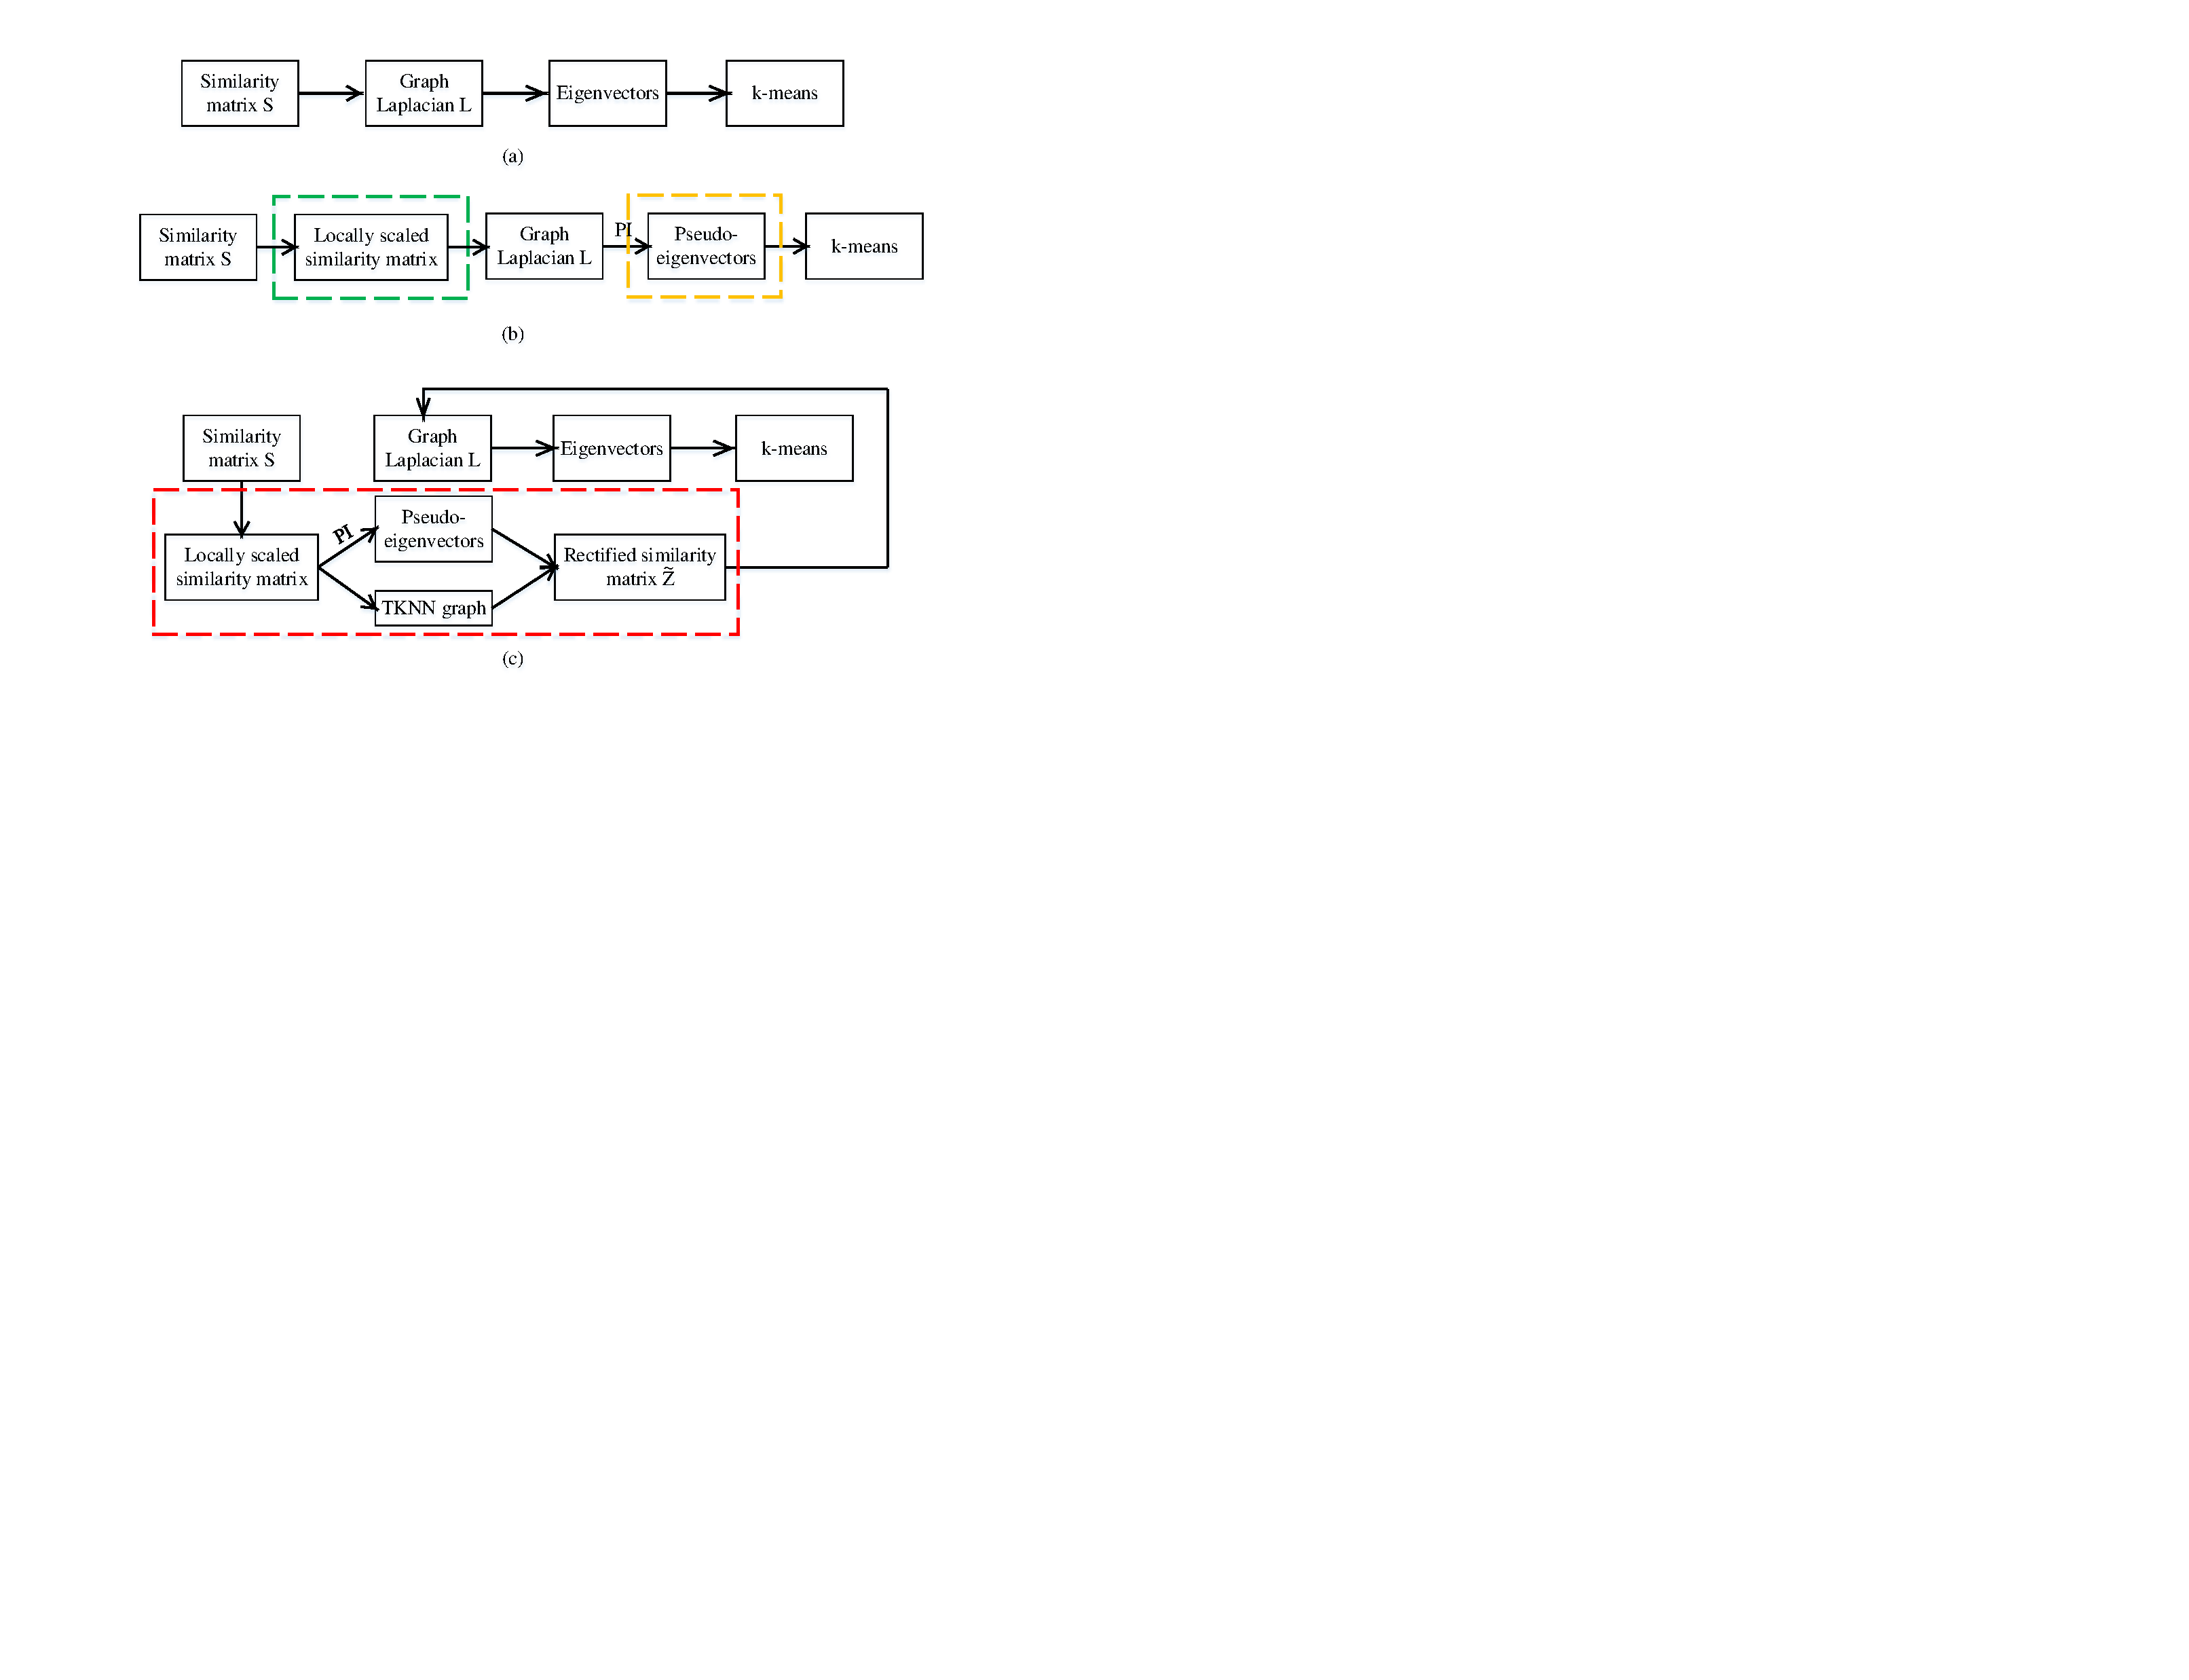
\includegraphics[width = 1.09\linewidth]{flow_graph3.pdf}
        \caption{The key steps of (a) basic spectral clustering; (b) with local scaling and PI; (c) ROSC}
        \label{figure:flow_graph}
\end{figure}
}

In this paper, we propose a novel semi-supervised classification algorithm on \textbf{H}eterogeneous \textbf{I}nformation \textbf{N}etworks via \textbf{G}raph \textbf{C}onvolution \textbf{N}ets, named HINGCN. Apart from hierarchical aggregation of node features, our model takes into account neglected edge information in TSSN methods as well.  by fine-tuning on pre-trained edge features


Our main contributions are:

\noindent$\bullet$
To compensate loss of information in shrinking homogeneous graph, we proposed a novel pre-process of edge feature. We also propose a novel fine-tuning mechanism for edge features, with limited computation power.

\noindent$\bullet$
We propose an 

\noindent$\bullet$
We conduct extensive experiments %using synthetic and real datasets 
to evaluate the performance of HINGCN
against $9$ other classification methods. 
Our results show that HINGCN performs very well against the competitors. 
In particular, it is very robust in that it consistently performs well over all the datasets tested. 
Also, it outperforms others by wide margins for datasets that are highly multi-scale. 

The rest of the paper is organized as follows.
%In Section~\ref{sec:preliminary} we give more details of spectral clustering and briefly 
%describe the power iteration method.
Section~\ref{sec:related} mentions related works on heterogeneous graph neural networks, graph embedding and described several semi-supervised classification algorithms.
Section~\ref{sec:algorithm} presents the HINGCN algorithm.
Section~\ref{sec:exp} describes the experiments and presents experimental results.
Finally, Section~\ref{sec:conclusion} concludes the paper.












